\chapter{CAP Theorem}

\section{Scalability of Elasticsearch}
A single node setup as seen in figure \ref{fig:singlenodesetup} corresponds to a cluster with only one node \autocite{elastic2019_10}. When storing an index in Elasticsearch the data gets split into shards. In figure \ref{fig:singlenodesetup} the only existing node contains 3 shards, where each shard is a primary shard containing the original data. In figure \ref{fig:clustersetup} the same data gets stored in an Elasticsearch cluster with three nodes. Now each primary shard gets duplicated with a replica shard. The shards get distributed between the nodes to balance the load of each node and reduce the risk of losing data should one node get destroyed \autocite{elastic2019_10}.

\begin{figure}[ht]
    \centering
    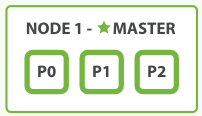
\includegraphics[width=0.33\textwidth]{image3.png}
    \caption{Single node setup \autocite{elastic2019_09}}
    \label{fig:singlenodesetup}
\end{figure}

\begin{figure}[ht]
    \centering
    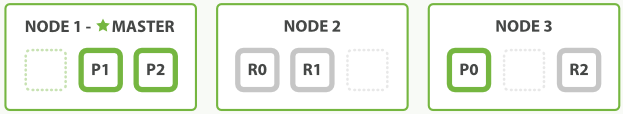
\includegraphics[width=1\textwidth]{image12.png}
    \caption{Cluster setup \autocite{elastic2019_09}}
    \label{fig:clustersetup}
\end{figure}

The size of the shards can be determined when creating the index. Choosing a suitable shard size is important to get the highest performance \autocite{dahlqvistc2018}. For example, if the whole data is in one big shard, a search query will take a comparatively long duration \autocite{dahlqvistc2018}. If the data gets divided over multiple shards, the same query can be applied to each shard and will be faster, because the query can run simultaneously on each shard. In the end, however, the results still have to be aggregated. This means having too many very small shards will increase the duration again \autocite{dahlqvistc2018}. Elasticsearch itself does not provide a fixed value for the size of a shard, they rather give some tips, like to keep the average shard size between 20GB and 40GB, but they recommend to always test what works best for each setup \autocite{dahlqvistc2018}.

Each Elasticsearch node can serve one or more purposes \autocite{elastic2019_10}. What purpose a node should serve can be set in the configuration file of each node \autocite{elastic2019_10}. In a single node setup this is not relevant, because the only existing node needs to fulfill every purpose. But in a big cluster it can make sense to have nodes dedicated to a single functionality to make sure that they are not strained too much \autocite{elastic2019_10}.

The different node types are:
\begin{itemize}
    \item \textbf{Master-eligible node} \\
    This node can be elected as the master, which controls the cluster \autocite{elastic2019_10}.
    \item \textbf{Data node} \\
    A data node stores the data and performs CRUD or search operations \autocite{elastic2019_10}.
    \item \textbf{Ingest node} \\
    Ingest nodes are used to apply a pipeline (serie of transformations or enrichments) to a document before indexing \autocite{elastic2019_10}.
    \item \textbf{Coordinating node} \\
    A request gets taken over by one node, that forwards the requests to the data nodes and then gathers the results. Each node can implicitly coordinate, but by disabling all other functionalities for a node, this node becomes a dedicated coordinator node \autocite{elastic2019_10}.
\end{itemize}

\section{Classification in the CAP Theorem}
The CAP Theorem is used to classify NoSQL databases, respectively distributed systems into Availability, Consistency and Partition Tolerance. According to the CAP theorem, each application can fulfill only two of the three mentioned attributes. Even if the classification is not so clear anymore since the theorem was set up \autocite{brewere2012}, it offers a possibility to compare different NoSQL databases.
 
The classification of Elasticsearch into the CAP Theorem is also not straightforward. On the Internet people provide answers for all the different combinations possible in the CAP Theorem \autocites{longn2014}{synhershkoi2014}. Elasticsearch itself provides no official statement on how they would classify their product. But based on the technical functionality of Elasticsearch and the example scenarios from \autocite{nathanir2019}, the following classification can be made:

When setting up Elasticsearch with no further configuration, the system is \textbf{AP}. 

This can be demonstrated by simulating a partitioning in a simple cluster consisting of 3 nodes as seen in figure \ref{fig:splitbrain}. Without configuration, each node is master-eligible. In addition each cluster has a property called \texttt{minimum\_master\_nodes}, which is set to one by default. This means that in the case of partitioning, each subcluster, even consisting of only one node, can choose itself as the new master. This is possible because it only needs to see one master-eligible node (itself) to conduct a election. As seen in figure \ref{fig:splitbrain}, the original cluster is now split into two independent clusters, where each continues to accept and process requests. Therefore Elasticsearch is available, but giving up on consistency. A so called split brain scenario has arisen. This can only be repaired by shutting down the smaller part of the cluster, so that this nodes can rejoin the bigger cluster. In this process the additional data of the restarted nodes is lost.

\begin{figure}[ht]
    \centering
    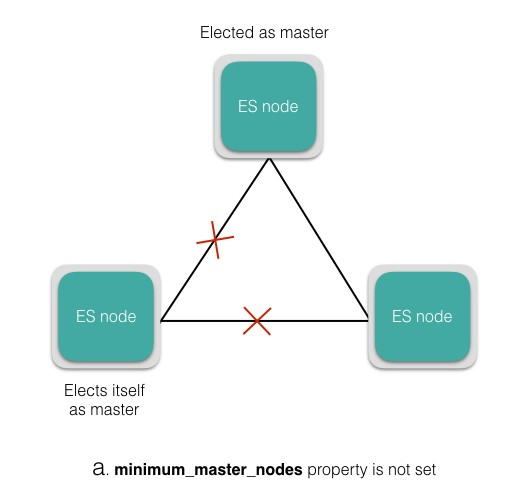
\includegraphics[width=0.5\textwidth]{splitbrain.png}
    \caption{Split brain scenario \autocite{nathanir2019}}
    \label{fig:splitbrain}
\end{figure}

After a configuration of the cluster (recommended by Elasticsearch) the system can be CP.

As already mentioned, there is a property called \texttt{minimum\_master\_nodes}. By setting this property to $(n/2)+1$, with $n$ being the number of master-eligible nodes, the scenario of a split brain can be prevented. Figure 7 shows the same cluster consisting of three nodes simulating a partitioning. The difference is that \texttt{minimum\_master\_nodes} is set to two. The isolated node therefore cannot select itself as master, since it does not see the required 2 nodes. Only the larger part of the cluster, consisting of the required 2 nodes, continues to accept and process requests. So in this case Elasticsearch gives up on availability and instead preserves consistency. After the partitioning is resolved, the single node will automatically rejoin the bigger cluster.

\begin{figure}[ht]
    \centering
    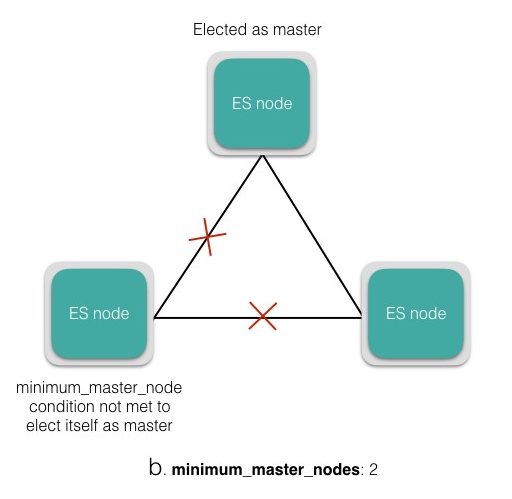
\includegraphics[width=0.5\textwidth]{nonsplitbrain.png}
    \caption{Non split brain scenario \autocite{nathanir2019}}
    \label{fig:nonsplitbrain}
\end{figure}

To conclude: Elasticsearch cannot be placed explicitly in the CAP theorem, because depending on the configuration, availability or consistency can be abandoned.
